% !TEX encoding = UTF-8 Unicode
\documentclass[a4paper,twocolumn,twoside]{article}
%%%%%%%%%%%%%%%%%%%%%%%%%%%%%%%%%%%%%%%%%%%%%%%%%%%%%%%%%%%%%%%%%%%
% Packages using
%%%%%%%%%%%%%%%%%%%%%%%%%%%%%%%%%%%%%%%%%%%%%%%%%%%%%%%%%%%%%%%%%%%
\ifx\pdfoutput\undefined
	\usepackage[dvips]{graphicx}
	\DeclareGraphicsExtensions{.eps}
\else
	\usepackage[pdftex]{graphicx}
	\DeclareGraphicsExtensions{.pdf,.jpg,.png,.mps}
	\pdfcompresslevel=9
\fi
\usepackage[utf8]{inputenc}
\usepackage[english]{babel}
\usepackage{indentfirst}
\addtolength{\topmargin}{-20mm}
\addtolength{\textheight}{10mm}
\usepackage{amsmath} % Added to get modern math environments
\usepackage{amssymb,amsfonts} %Added to get math
\usepackage{amsthm} % Added to get theorems
\usepackage{natbib} % Added to get better bibliography
\usepackage{wrapfig}

\usepackage{url}
% Special hack below to break the URL!
\def\UrlBreaks{\do\.\do\@\do\\\do\/\do\!\do\_\do\|\do\;\do\>\do\]%
 \do\)\do\,\do\?\do\'\do+\do\=\do\#\do\i\do\m\do\t\do\a\do\x}%
\urlstyle{rm} %
\usepackage[bookmarks=true,bookmarksnumbered=true,hypertexnames=true,breaklinks=true,colorlinks=true]{hyperref}
\hypersetup{
pdfauthor = {Torbj\"{o}rn E. M. Nordling},
pdftitle = {Information Retrieval and Processing--Setup of a Full Text System Implementing Automatic Metadata Extraction and Visualisation},
pdfsubject = {Technical Report},
pdfkeywords = {Information retrieval, Metadata}}

% Headers and footers (must be after the document settings)
\usepackage{fancyhdr} %Custom header package
\pagestyle{fancy} %Turn on fancy headers
\fancyhead{} %Clears default layout
\fancyfoot{} %Clears default layout
\fancyhead[LO,RE]{\small \normalfont \leftmark} %Adds section headline to header
\fancyhead[LE,RO]{\slshape \rightmark} %Adds subsection headline to header
\fancyfoot[LO,RE]{\href{http://www.nordlinglab.org/ScientificInformation}{nordlinglab.org/ScientificInformation}}
\fancyfoot[RO,LE]{Information Retrieval and Processing}
\fancyfoot[CO,CE]{\thepage}
\renewcommand{\headrulewidth}{0.4pt} %Header line
\renewcommand{\footrulewidth}{0.4pt} %Footer line

%%%%%%%%%%%%%%%%%%%%%%%%%%%%%%%%%%%%%%%%%%%%%%%%%%%%%%%%%%%%%%%%%%%

\begin{document} 
	
	\title{Information Retrieval and Processing--Setup of a Full Text System Implementing Automatic Metadata Extraction and Visualisation}
	\author{Chinweze Ubadigha, Dexter Chen, Eric Chang, Eric Lee, Feng-Chun Hsia,\\
		 I-Chieh Lin, Jacky Wu, Jim Lan, Karthick Mani, Yu-chemg Chen,\\ 
		 Piyarul Hoque,
		  Torbjörn E. M. Nordling}  % Please add your name here in alphabetic order (except Prof. N who is last)
	\maketitle   
	
	\section{Introduction}
	\label{Introduction}
	
	This technical report contains both general information on the state of the scientific information retrieval and processing art and a description of the \href{https://bitbucket.org/nordron/nordron-sciinfo}{Nordron-SciInfo} software package for information retrieval and processing. 
	This report was written by all participants of the \emph{Scientific Information Gathering and Processing for Engineering Research} course lead by Prof. Nordling at the National Cheng Kung University in the spring semester 2016. The main objectives of the course is to teach the students state of the art information retrieval and processing methods, project management, and technical writing by doing a project on implementation of some methods for retrieval and processing of full text scientific articles. The result of the student project is described in this report.
	
	\subsection{Aim and project structure}
	\label{aim}

	The whole project was separated into three parts, each with a responsible team:
	\begin{enumerate}
		\item Create a data base of open access full text articles (Team Wolverine).
		\item Create a complementary XML like structure for metadata that contains all information in the PDF and can be show in Utopia (Team Eagle unit).
		\item Automatic creation of metadata/markup by use of natural language processing of full text articles (Team Union).
		%\item Automatic creation of links from full text articles to external sources (Team Hanky Phanky).
	\end{enumerate}
	
	\section{Background}
	\label{Background}

	%%%%%%%%%%%%%%%%%%%%%%%%%%%%%%%%%%%%%%%%%%%%%%%%%%%%%%%%%%%%%%%%%%%
% Background
% Team:
% Wolverine
% Members: 
% Dexter Chen, Eric Chang, Eric Lee, Jacky Wu, Karthick Mani, Kenvin Lo, Yu-cheng Chen
% Relative files:
% Main.tex, Background_Wolverine.tex, Library.bib, Wolverine_Background_Chart_1.png
% Note: 
% Do not compile this file compile Main.tex to get the pdf file instead.
%%%%%%%%%%%%%%%%%%%%%%%%%%%%%%%%%%%%%%%%%%%%%%%%%%%%%%%%%%%%%%%%%%%
	
\subsection{Information retrieval on existing database}
\textit{\footnotesize Author:Dexter Chen, Eric Chang, Eric Lee, Jacky Wu, Karthick Mani, Kenvin Lo, Yu-cheng Chen.}\\

We live in the time where technologies evolve beyond our imagination.
Information growth in a exponential rate according to \cite{Tague1981}, thus we can't rely on the old fashion ways to find data. 
We need new information retrieval methods to handle such a big amount of data.
But most of the information retrieval methods such as search engine can't really search everything on the web. 
They can only search the data that has been captured into the database according to \cite{Grehan2002}. 
Thus, we need to create a database to store these data and automatically update them frequently.

There are several online libraries currently available for us to get the academic articles we need.
And they can be roughly divided into three group according to the way they store articles base on the division used by National Taiwan University Library.

\paragraph{Index libraries}

	These kind of libraries stores the index and abstract of the articles.
	They don't provide the full-text documents directly, but may give the linkage to the publisher websites of articles.
	And can be categorized by the type of articles they include.
	
	\begin{itemize}
		
		\item\textbf{Comprehensive topics}\\Libraries such as Web of Science, Scopus...
		\item\textbf{Specialized topics}\\Libraries such as Compendex, BIOSIS Previews, PubMed...
		
	\end{itemize}
	
\paragraph{Publisher libraries}

	These libraries are created by the publishers themselves, so they provide the newest and complete documents directly.
	And can also be categorize by the type of articles they include.
	
	\begin{itemize}
		
		\item\textbf{Comprehensive topics}\\Libraries such as Science Direct, Springer Link, Wiley Online Library...
		\item\textbf{Specialized topics}\\Libraries such as Nature.com, Emerald Management Xtra, IEEE Xplore...
		
	\end{itemize}
	
\paragraph{Aggregator libraries}

	These libraries do not publish the articles by themselves, but they still sometimes provide the full-text articles to the user.
	The way they do this is to negotiate with some of the publisher libraries and get the authorization of the articles.
	Libraries such as EBSCOhost, ProQuest, JSTOR...

The comparison between three kinds of library can be found on Figure \ref{WBC1}. 
On the next section we'll discuss about more details about some of the existing libraries.

\subsubsection{Introduction to several libraries }\todo{Consider to change the title.}

\begin{enumerate}
	
	\item\textbf{PubMed}
	\setlength{\parindent}{1em}
		
	 PubMed is a free library which is used for searching reference papers and abstracts related to the biomedical topics.
	 PubMed’s design philosophy is based on full-text XML files, which are readable by both the machines, humans and moreover technology independent.
	 PubMed is classified into Index libraries, which is the prime reason that it won’t be able to provide full text in some papers.
	 For the type of database used by PubMed is Microsoft SQL server, which is a relational database to store all of the archives such as XML, images, PDF files supplementary, etc. \todo{Good that you start by describing what it is and then tell how it is built.}
		
	\item\textbf{IEEE Xplore}
	\setlength{\parindent}{1em}
	
	IEEE Xplore is a scholarly research library formerly known as IEEE/IET Electronic Library (IEL).
	The IEEE is an acronym for Institute of Electrical and Electronics Engineers, which is one of the leading standard organizations in the world.
	More than 3.5-million full-text documents in the field of electrical, engineering, computer science and electronics are provided in this library. 
	
	The front and user interface of IEEE library present the information on the screen, including the latest Angular, Jquery, HTML 5, CSS, etc.\todo{You mean it is implemented using these techniques. Please don't use etc. when you describe how something is built and do it in this context.} 
	Most of the HTML for PDF, either it is for journal (conference) articles or standards get dynamic transformations real time and served through MarkLogic.
	Endeca, which is an Oracle product powers Xplore searches, is used in the search layer.
	All PDF files are fed through Endeca system.
	Endeca servers will provide the matching documents and Xplore platform presents it on the screen to the user.
	And all the content is stored in oracle metadata which will be consumed by Endeca, MarkLogic Authentication, and Authorization services.
	
	\item\textbf{EBSCOhost}
	\setlength{\parindent}{1em}
	
	EBSCOhost is a popular reference which authorizes users to gain a great many full-text articles from proprietary databases.
	EBSCO Information Services, headquartered in Ipswich, Massachusetts, 
    is a division of EBSCO Industries Inc., 
    the third largest private company in Birmingham, Alabama, with annual sales of nearly $2 billion according to the BBJ's 2013 Book of Lists.

    EBSCO offers library resources to customers in academic, medical, K–12,  
    public library, law, corporate, and government markets. Its products include EBSCONET, a complete e-resource management system, 

    and EBSCOhost, which supplies a fee-based online research 
    service with 375 full-text databases, a collection
    of 600,000-plus ebooks, subject indexes, point-of-care 
    medical references, and an array of historical digital archives.

    In 2010, EBSCO introduced its EBSCO Discovery Service (EDS) to institutions,
    which allows searches of a portfolio of journals and magazines

	
	\item\textbf{Comparison Xplore}
	\setlength{\parindent}{1em}
	
	PubMed is a free library which contains many databases, like Medline, PreMedline and Publisher Supplied Citations.
    One can also access Medline through EBSCOhost. 
    Medline is the largest subset of PubMed. 
    You may limit your search to Medline only in PubMed. 
    Both of them are built by National Library of Medicine. 
    In contrast to other two libraries, the advanced search of PubMed is weak. 
    It do not show citation times or further information.
    The documents in PubMed are almost related to the biomedical topics.
    IEEE contains more than one third documents in the field of electrical, engineering, computer science and electronics.
    And EBSCOhost PubMed is a free search engine accessing primarily the MEDLINE 
    database of references and abstracts on life sciences and biomedical topics. 
    

\end{enumerate}

\todo[inline]{You need to add at least one library example of each library type, since you started with different types. Otherwise you could have focused on one type and motivated the focus. For the libraries containing articles you should add several since you are building one. You should also discuss the database techniques, including alternative ones to the used ones, such as MongoDB, Hadoop, etc. Try to compare features.}

\begin{figure*}[htb]
	\begin{center}
		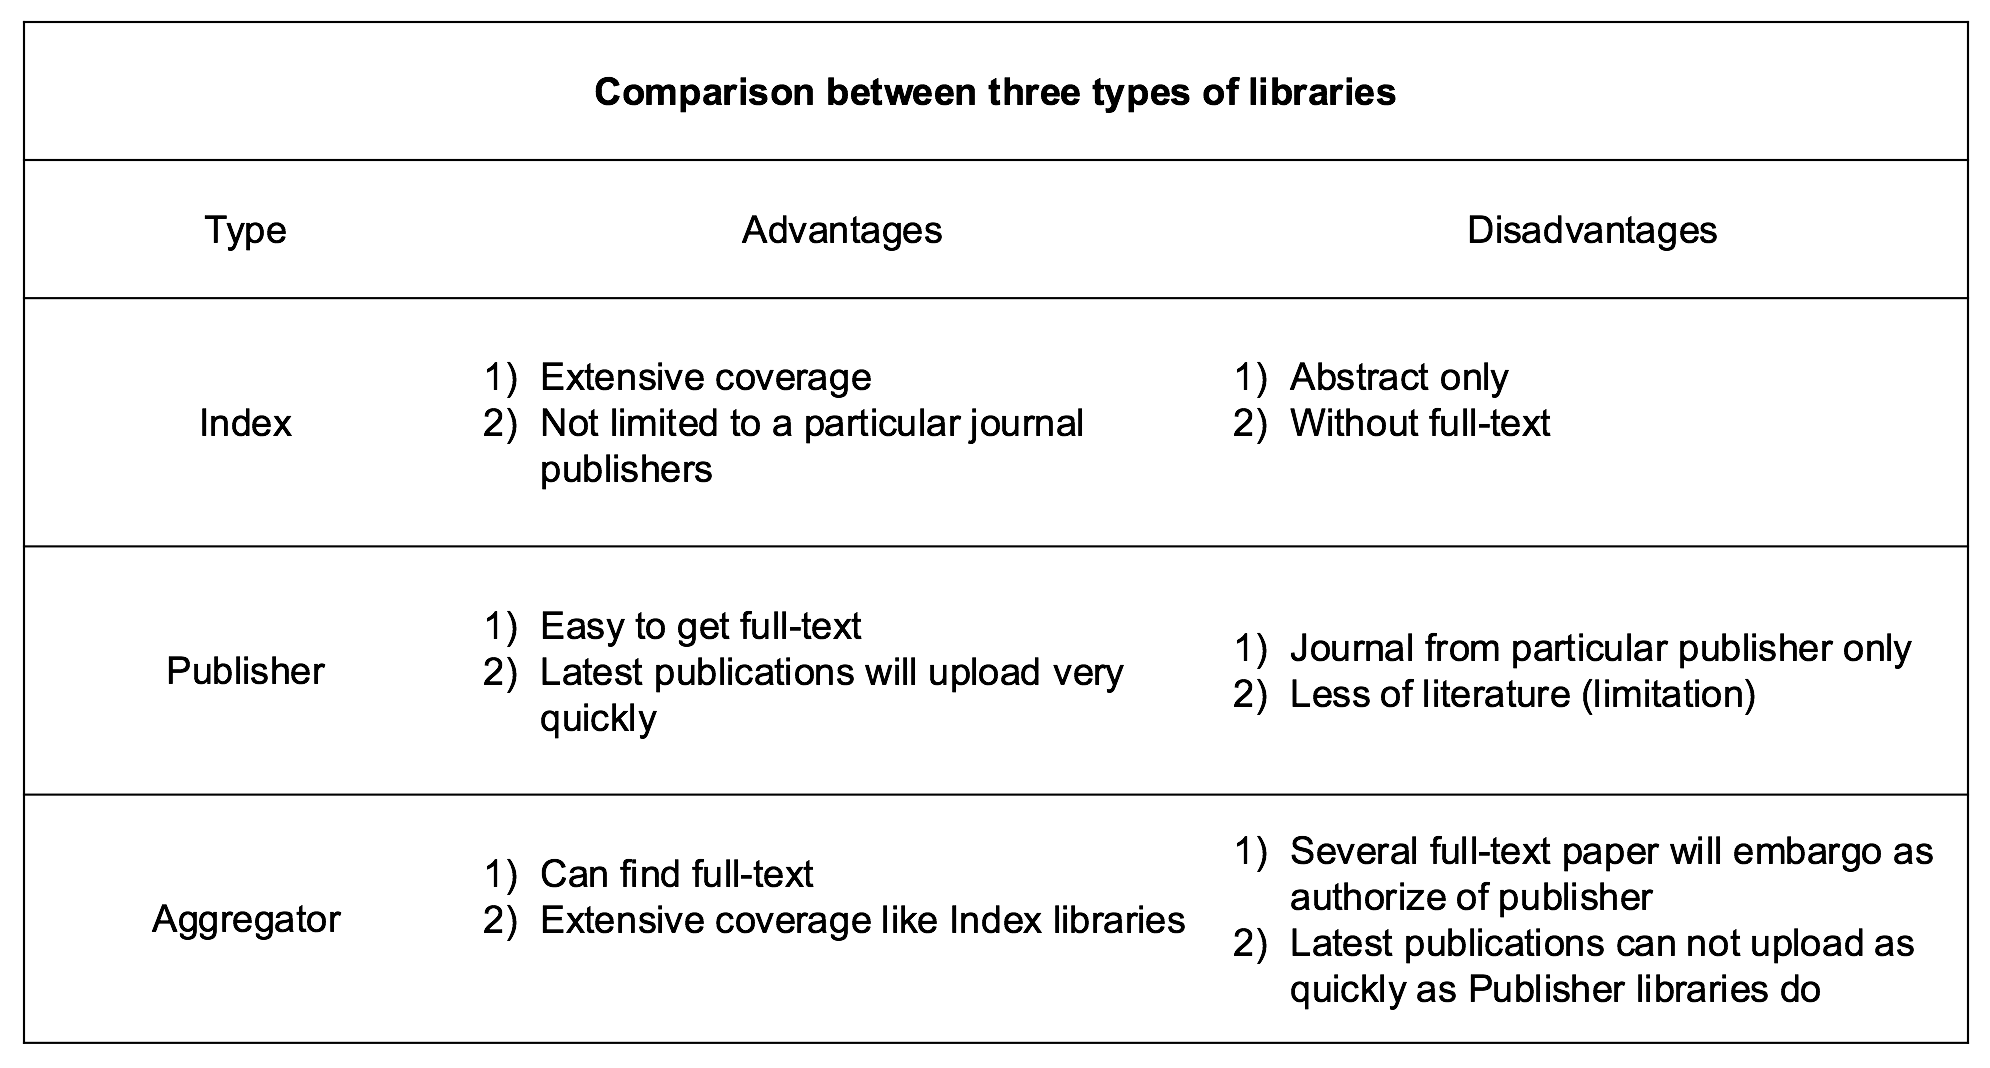
\includegraphics[width=0.8\textwidth]{Wolverine_Background_Chart_1}
	\end{center}
	\caption{Comparison between three types of libraries.\label{WBC1}}
\end{figure*}
\newpage

	%%%%%%%%%%%%%%%%%%%%%%%%%%%%%%%%%%%%%%%%%%%%%%%%%%%%%%%%%%%%%%%%%%%%%%%%%%%%%%%%%%%
% Team:
% EagleUnit
% Members: 
% Chinweze Ubadigha, Feng-Chun Hsia, Henry Peng, I-Chieh Lin, Jones Hou, Piyarul Hoque, Ray Chang
% Relative files:
% Main.tex, Background_EagleUnit.tex, Library.bib, EagleUnit_Background_Chart_1.png
% Note:
% Do not compile this file compile Main.tex to get the pdf file instead.
%%%%%%%%%%%%%%%%%%%%%%%%%%%%%%%%%%%%%%%%%%%%%%%%%%%%%%%%%%%%%%%%%%%%%%%%%%%%%%%%%%%
\subsection{XML metadata structure}
\textit{\footnotesize Author:Chinweze Ubadigha, Feng-Chun Hsia, Henry Peng, I-Chieh Lin, Jones Hou, Piyarul Hoque, Ray Chang.}\\

Our responsibility is building a metadata schema which contains all information in a PDF and then edit it in an XML structure. This article provides an overview of metadata standards which are related to our responsibility. A number of metadata schemas in use nowadays are reviewed, including MODS, METS, METS+MODS+PREMIS, MARC21, MARC XML, Dublin Core, and  their pros and cons. Finally, we compare these schemas by examining the characteristics and unique features of them. We are able to rank them and suggest the optimum standard to build our XML structure. XML is a markup language that defines a set of rules for encoding documents in a format,  which is both human-readable and machine-readable. It is widely used for the representation of arbitrary data structures, such as those used in web services.

Metadata is defined as the "data about data" or alternatively "information about information". In practice, metadata summarizes basic information of data for the organization and management of documents. It can be accessed manually or by automatic information processing and coding. \cite{underwood2003xml}.

The metadata schemas can be classified into three types \cite{dempsey1997specification}:
\begin{itemize}
	\item Simple formats: it includes relatively unstructured data, typically automatically extracted from resources and indexed for searching. The data has little explicit semantics and does not support searching by field, such as Lycos, Altavista, Yahoo, etc.
	\item Structured formats: it includes data which contains full enough description to allow a user to assess the potential utility or interest of a resource without having to retrieve it or connect to it. The data is structured and supports fielded searching, such as Dublin Core, IAFA templates, RFC 1807, SOIF, LDIF.
	\item Rich formats: it includes fuller descriptive formats which may be used for location and discovery, but also have a role in documenting objects or, very often, collections of objects, such as ICPSR, CIMI, EAD, TEI, MARC.
\end{itemize}

XML (Extensible Markup Language) is the universal format for the encoding and exchange of structured documents and data. There are no predefined tags and document structures in XML. In other words, the XML provides structural capabilities that HTML lacks, making it easy to achieve the principles of modularity and extensibility. The XML schema specification defines a schema language that allows for the specification of application profiles that will increase the prospects for interoperability \cite{duval2002metadata}. Our work is to build a metadata schema in XML structure. The following sections will introduce the different schemas as mentioned previously.

%%%%%%%%%%%%%%%%%%%%%%%%%%%%%%%%%%%%%%%%%%%%%%%%%%%%%%%%%%%%%%%%%%%%%%%%%%%%%%%%%%%
% 1. Different standards of metadata
%%%%%%%%%%%%%%%%%%%%%%%%%%%%%%%%%%%%%%%%%%%%%%%%%%%%%%%%%%%%%%%%%%%%%%%%%%%%%%%%%%%

\subsubsection*{Different standards of metadata}
\label{sec:mets}
There are various types of standards that describes the metadata in different fields and applications. Listed in the following are five different standards with a brief introduction to each one.

\begin{figure*}		
	\begin{center}
		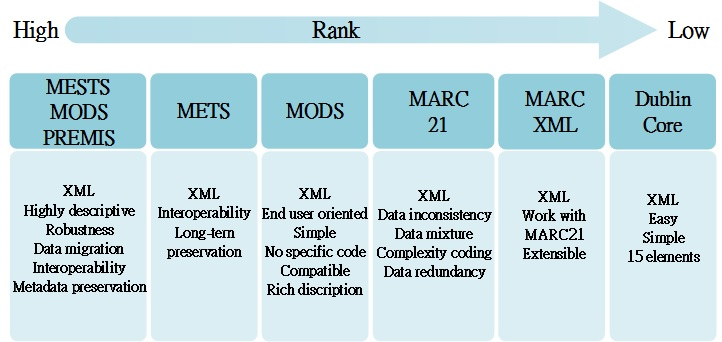
\includegraphics[width=1.8\columnwidth]{EagleUnit_Background_Chart_1}
	\end{center}
	\caption{Overview and hierarchical ranking of metadata standards and their individual features}
\end{figure*}

\begin{enumerate}
	\item METS\\
	{\bf Introduction}\\
	Metadata Encoding and Transmission Standard (METS) similar to XML encoding format for storing the descriptive, administrative, structural and behavioral metadata needed to manage complex digital objects in open and standardized way.
	
	In 1990s, Making of America II (MOA2) project was proposed to share vision between national digital libraries which provides a means for the Digital Library Federation (DLF) to investigate, refine, and recommend metadata elements and encodings used to discover, display, and navigate digital archival objects. MOA2 DTD was created to test MOA2 project.
	
	However, MOA2 DTD was limited in several ways. It provided no flexibility in terms of the exact metadata elements to be used for descriptive, administrative and structural metadata. Also, limited in scope to support for text and still image materials and no attempt to support time-based media such as audio or video materials. To solve those problems led to the creation of METS.
	
	{\bf Advantages}
	\begin{enumerate}
		\item METS to facilitate the exchange and interoperability of digital library objects across digital library systems.
		\item Provide support a practical and flexible packaging mechanism for the long-term preservation of digital library objects.
		\item The METS standard can be considered one of many efforts to try to determine, for one particular community, how complex sets of data and metadata might best be encoded to support both information exchange and information longevity.
	\end{enumerate}	
	{\bf Disadvantages}
	\begin{enumerate}
		\item METS has gone some distance towards achieving these design goals, it is not in itself a guarantee of interoperability.
		\item There are some obvious practical difficulties in using METS for the long-term preservation of digital objects.
	\end{enumerate}
	{\bf Conclusion}\\	
	
	%%%%%%%%%%%%%%%%%%%%%%%%%%%%%%%%%%%%%%%%%%%%%%%%%%%%%%%%%%%%%%%%%%%%%%%%%%%%%%%%%%%
	\item MODS\\
	{\bf Introduction}\\
	Metadata Object Description Schema (MODS) was developed by the Library of Congress' Network Development and MARC Standards Office in 2002. It is a bibliographic element set for multiple purposes, especially for library applications. As an XML schema, it is not only able to carry the selected data from existing MARC 21 records but to enable the creation of original resource description records. It includes a subset of MARC and uses language-based tags rather than numeric ones. In some cases regrouping elements are from the MARC 21 bibliographic format. It released the third version (version 3.6) in May 2015. MODS is expressed using the XML of the World Wide Web Consortium. The standard is maintained by the MODS Editorial Committee with support from the Network Development and MARC Standards Office of the Library of Congress.\\
	
	MODS is an XML schema which is guidelines a resource description for encoding, as well as exchange and management descriptions of encoding.\\
	
	Elements of MODS generally inherit the MARC, some data has been repackaged; in some cases what is in several data elements in MARC may be brought together into one in MODS. Also, MODS does not assume any specific cataloging code.\\ It is used as an extension schema to METS (Metadata Encoding and Transmission Standard), as a representing a simplified MARC record in XML.
	
	{\bf Advantages}
	\begin{enumerate}
		\item The element set is richer than Dublin Core.
		\item The element set is more compatible with library data than ONIX.
		\item The schema is more end user oriented than the full MARCXML schema.
		\item The element set is simpler than the full MARC format. 
	\end{enumerate}	
	{\bf Disadvantages}
	\begin{enumerate}
		\item An original MARC 21 record converted to MODS may not convert back to MARC 21 in its entirety without some loss of specificity in tagging or loss of data.
		\item In some cases if reconverted into MARC 21, the data may not be placed in exactly the same field that it started in because a MARC field may have been mapped to a more general one in MODS.
		\item MODS does not include business rules for populating the elements.
		\item Additional instructions would need to be provided for conversion details.
	\end{enumerate}
	{\bf Conclusion}\\
	MODS has a high level of compatibility with MARC records because it inherits the semantics of the equivalent data elements in the MARC 21 bibliographic format. It may be used for the original resource description that allows for rich description that is generally compatible with existing library data and is expressed in XML syntax. Because it includes a subset of MARC fields and repackages some of them, it is particularly useful for technician input.\\
	An additional use of MODS is as an extension schema for descriptive metadata for the METS object.
	
	%%%%%%%%%%%%%%%%%%%%%%%%%%%%%%%%%%%%%%%%%%%%%%%%%%%%%%%%%%%%%%%%%%%%%%%%%%%%%%%%%%%
	
	\item METS+MODS+PREMIS\\
	{\bf Introduction}\\
	The first developed of digital repositories of the British Library's e-journal system was the combination of METS, MODS and PREMIS..\cite{Dappert2008} It exploited the METS structural, PREMIS preservation and MODS descriptive metadata to form a robust metadata structure. The Metadata Encoding and Transmission Standard (METS) is an XML document that can package the metadata of a digital resource: the descriptive, administrative, structural, rights and other data needed for retrieval and preserving of a digital resources.\cite{Guenther2003} In other words it can be referred as a metadata storing and communication standard. The METS wrapper has up to seven major subsections: "a METS Header (metsHDR), a Descriptive Metadata Section (dmdSec), an Administrative Metadata Section (amdSec), a File Section (fileSec), a Structural Map (structMap), Structural Links (structLink), and a Behavior Section (behaviorSec)" these form the basic structure of METS. The Structural Map is the most important subsection and must be included in a METS document.\cite{Cheslow2014} These subsections have elements that provide the means for describing in detail the digital objects. The Structural Map defines a hierarchical structure such that using METS pointers users of the digital library object can easily navigate through it . One great advantage of METS is that it provides a flexible framework for modelling different document types and scenarios.\cite{Dappert2008}
	The Metadata Object Description Standard (MODS) provides ways to describe objects and has a high level compatibility with MARC. Among other XML metadata standard it is an alternative between a simple metadata format (such as Dublin Core) which has a minimum of fields and little or no substructure, and a very detailed format (such as MARC 21) with many data elements having various structural complexities.\cite{Guenther2003}
	The PREservation Metadata Implementation Strategies (PREMIS) is an administrative metadata schema used for the preservation of digital resources.\cite{Cheslow2014} With the rapid changes in technology, digital objects including its metadata are bound to go obsolete at some time in the future. PREMIS was created to set standards that will ensure long term usability and preservation of digital resources.
	
	{\bf Why METS+PREMIS+MODS? }\\
	To understand metadata needs, whuch is important to understand the data production and structures. Structuring digital objects particularly e-journals present two main difficult problems. 
	First, e-journals are structurally complex. New issues are released in intervals for each journal title. These may contain a varying number of articles and other publishing matters having a variety of formats. Second, the production of e-journals are outside the control of the digital repository and done without the benefit of standards for the structure of file formats, metadata formats and vocabulary, publishing schedules, etc.\cite{Dappert2008}
	As a means to solve these problem, METS provides a robust and flexible way to define digital objects. The MODS on the other hand, provides ways to describe digital objects and can be built on a MARC. Finally the PREMIS provides ways to describe digital objects and processes that are essential for digital preservation. Also, these three metadata standards are all built on an XML schema.\cite{Dappert2008}
	Details on how to implement these three metadata standards to form a robust metadata structure or archive can be found in "Using METS, PREMIS and MODS for Archiving eJournals".\cite{Dappert2008} Though there are different ways to implement these schema only one was discussed in the aforementioned literature.
	
	{\bf Advantages}
	\begin{enumerate}
		\item Interoperability: According to Hafezi et al on their survey of Iranian digital library, most of the bibliographic data comprises of 82\% XML and 64\% MARC formats. Given these statistics, METS+PREMIS+MODS can be considered interoperable since they all can be implemented in these formats.\cite{AlipourHafezi2013}					
		\item XML Schema: Considering our given responsibility and the easiness of implementing XML, METS+PREMIS+MODS is among the right choice. 
		\item Metadata Preservation: The inclusion of PREMIS in METS provided the metadata preservation feature which single metadata standard cannot provide.
		\item Highly descriptive metadata: The MODS used in structuring the descriptive metadata in METS provided a highly descriptive metadata structure.
		\item Data migration: Because METS is flexible and contains header for easy transmission it is very easy to deploy this metadata structure to a different system.
		\item Robustness: This schema is considered robust by the virtue of containing the features of three different metadata standard.
	\end{enumerate}	
	{\bf Disadvantages}
	\begin{enumerate}
		\item Easiness: This schema is not ease to build compared to single metadata structure.
		\item Redundancy: Some of the metadata stored in the METS were also stored in the PREMIS to improve preservation.
		\item Update: The digital object in the repository are write-once in order to support archival authenticity and track digital object provenance, thus in-situ update is not possible. To update another version of the Archival information package has to be added.
	\end{enumerate}
	{\bf Conclusion}\\
	METS is an excellent metadata schema for use with digital libraries and will become more robust when combined with MODS for descriptive metadata and PREMIS for preservation metadata. Also, with a minimal knowledge of XML, METS is relatively easy to implement and the Library of Congress provides great resources to help implement METS.
	Our mission is to create a better metadata structure that can stand the test of time. Bearing this in mind and considering the metadata standards mentioned above, the combination of METS, MODS and PREMIS possesses the features that will resolve the limitations of present day information retrieval systems.
	
	%%%%%%%%%%%%%%%%%%%%%%%%%%%%%%%%%%%%%%%%%%%%%%%%%%%%%%%%%%%%%%%%%%%%%%%%%%%%%%%%%%%
	\item MARC 21\\
	{\bf Introduction}\\
	The Library of Congress Network Development and MARC Standards is developed a framework for working in MARC data in a XML environment. The MARC XML schema are not need to be edited to reflect of minor changes to MARC21. The schema retains the semantics of MARC.\\
	This information has been made in several areas and fields, one of these the bibliographic domain, where this is guided by instruments, principles, models and technologies. With the metadata standards used in this field, the MARC formats 21, with origins in the 1960s Considering the widespread use of these standards are, the objective of\\
	highlight the purposes that led to the creation of MARC formats 21. Which is carried out a literature review on the origin of MARC and its development in the MARC 21 and the coding records. Thus it is presented coding with XML and the MARCXML schema, as well as criticism of the MARC formats 21. It follows that, despite the criticism, the MARC formats 21 are still widely used and disseminated, and that despite the advantages offered by XML, encoding with the ISO 2709 standard. \\
	It is important to note that the MARC 21 is a data exchange format, which tells how import or export successfully occur the bibliographic and cataloging record and should be described, but the catalog data model should not necessarily be structurally organized in the same format as a MARC21 record. \\
	When the technological development will start with direct and indirect implications for informational resource representation activities and exchange of cataloging data. We hoped that the MARC formats 21, on development and on their encodings has contributed to the area of Information Science. \\
	But now-a-day the standards are the Metadata Object Description Schema (MODS) (Metadata Scheme for description of object) and the Metadata Authority Description Schema (MADS), both created for use with XML and specified by XML schemas.
	
	{\bf Advantages}
	\begin{enumerate}
		\item Data inconsistency: The same type of data is recorded in different fields / subfields of different forms.
		\item Data redundancy: the same data is recorded in more than one field / subfield, sometimes coded way, sometimes literally.	
		\item Data mixture and their attributes.
		\item Extreme complexity in coding.
	\end{enumerate}	
	{\bf Disadvantages}
	\begin{enumerate}
		\item Problems due to shared cataloging environment for which MARC 21 was designed.
		\item Problems caused or partially caused by MARC 21 and that perhaps can be solved in the data migration process to a new standard of data structure in the future.
	\end{enumerate}
	
	{\bf Validation of MARC21 data}
	\begin{enumerate}
		\item Basic XML validation according to the MARC XML Schema
		\item Validation of MARC21 tagging (field and subfield)
		\item Validation of MARC record content, e.g., coded values, dates, and times.
	\end{enumerate}
	
	{\bf Conclusion}\\
	The MARC formats 21 are still widely used and disseminated for the exchange of cataloging data in digital environments. Despite the advantages offered by coding the XML, including the development of software for processing MARC 21 records still persists.\\
	Together with efforts to use XML - coding in MARC records 21, LC is designed metadata standards which have alternatives to traditional formats. Among these standards are the Metadata Object Description Schema (MODS) (Metadata Scheme for description of object) and the Metadata Authority Description Schema (MADS), both created for use with XML and specified by XML schemas.\\
	The MODS and MADS have great compatibility with traditional formats MARC 21, although, in general, do not allow the data record with the same level of specificity given by the MARC formats 21.\\
	The MODS, due to its high compatibility with the MARC format 21 for Bibliographic Data can be chosen by libraries as a metadata standard for describing information resources.

	%%%%%%%%%%%%%%%%%%%%%%%%%%%%%%%%%%%%%%%%%%%%%%%%%%%%%%%%%%%%%%%%%%%%%%%%%%%%%%%%%%%	
	\item MARCXML\\
	{\bf Introduction}\\
	To make up the less of internet compatibility of MARC 21, the Library of Congress developed an XML schema based on it. Which the schema is the MARCXML standard. The purpose of MARCXML is to build a metadata format with a simple, extensible and flexible structure, which can be presented in XML stylesheets. Since MARCXML was design to converged data from MARC 21, the structure and performance are very similar between these two standards.\\
	{\bf Advantages}
	\begin{enumerate}
		\item Used in XML directly.
		\item Easily work with MARC 21 system.
	\end{enumerate}	
	{\bf Disadvantage}
	\begin{enumerate}
		\item The disadvantage of MARC 21 can be almost totally found on MARCXML, except the ability of internet application.
	\end{enumerate}
	{\bf Conclusion}\\
	Since our responsibility is to construct an XML schema, MARCXML will be a good choice if MARC 21 becomes the standard to be worked with.
	
	%%%%%%%%%%%%%%%%%%%%%%%%%%%%%%%%%%%%%%%%%%%%%%%%%%%%%%%%%%%%%%%%%%%%%%%%%%%%%%%%%%%
	\item Dublin Core\\
	{\bf Introduction}\\
	Dublin Core provides very simple but efficient sets of metadata.
	Dublin Core’s four main principles are high flexibility, clear and easy to understand gereral connotation, global, easy to produce or maintain.
	There are fifteen core elements. These simple elements can be further defined to generate more detailed metadata.\\
	The original Dublin Core metadata element sets are as follow:
	1. Title 2. Creator 3. Subject 4. Description 5. Publisher 
	6. Contributor 7. Date 8. Type 9. Format 10. Identifier
	11. Source 12. Language 13. Relation 14. Coverage 15. Rights.
	\cite{NISO2012}
	
	{\bf Advantages}
	\begin{enumerate}
		\item Encourage authors and publishers to provide Metadata in the type that can be automatically collected by resource discovery tools.
		\item Encourage web publishing tool that contains element of the Metadata module to be founded, which further simplify the creation of Metadata records.
		\item DC records can be the basis of more detailed cataloging records.
		\item After the DC becomes the standard, Metadata records can be understood by the user.
	\end{enumerate}	
		
	{\bf Disadvantages}
	\begin{enumerate}
		\item There are no cataloging rules that determine how data will be filled in. So if I write " Contributor: Sam Smith ", I can also write "contributor = Smith, Sam.". It means that there is no consistency across different uses of Dublin Core.
		\item Does'nt work well for data conversion.
		\item Data values in non-mappable space will be left out, especially when a source schema has a richer structure than the target schema. E.g., from METS to Dublin core.
	\end{enumerate}
	{\bf Conclusion}\\
	Because there are no cataloging rules, it makes Dublin core easy to use by anyone. On the other hand, this is something that goes against the article cataloging.
	%%%%%%%%%%%%%%%%%%%%%%%%%%%%%%%%%%%%%%%%%%%%%%%%%%%%%%%%%%%%%%%%%%%%%%%%%%%%%%%%%%%
		
\end{enumerate}
	
\newpage % Ends the current page and causes all figures and tables to be printed






	%%%%%%%%%%%%%%%%%%%%%%%%%%%%%%%%%%%%%%%%%%%%%%%%%%%%%%%%%%%%%%%%%%%%%%%%%%%%%%%%%%%
% Team:
% Union
% Members: 
%  
% Relative files:
% 
% Note:    
% 
%%%%%%%%%%%%%%%%%%%%%%%%%%%%%%%%%%%%%%%%%%%%%%%%%%%%%%%%%%%%%%%%%%%%%%%%%%%%%%%%%%%

\subsection{Automatic creation of metadata}
\textit{\footnotesize Author:Bernie Huan, Hoang Tan, Jim Lan, Kenny Hsu, Wei, Tan Phat.}\\

We're producing a program which automatically generate metadata such as authors' name, date of publishing, name of articles... and more importantly auto-abstract for full text articles

We are interested in features for either more convenient use of the program or improving precise data generation
There are 5 related problems.

\begin{figure}
	\caption{The process of metadata creation}
\begin{center}
	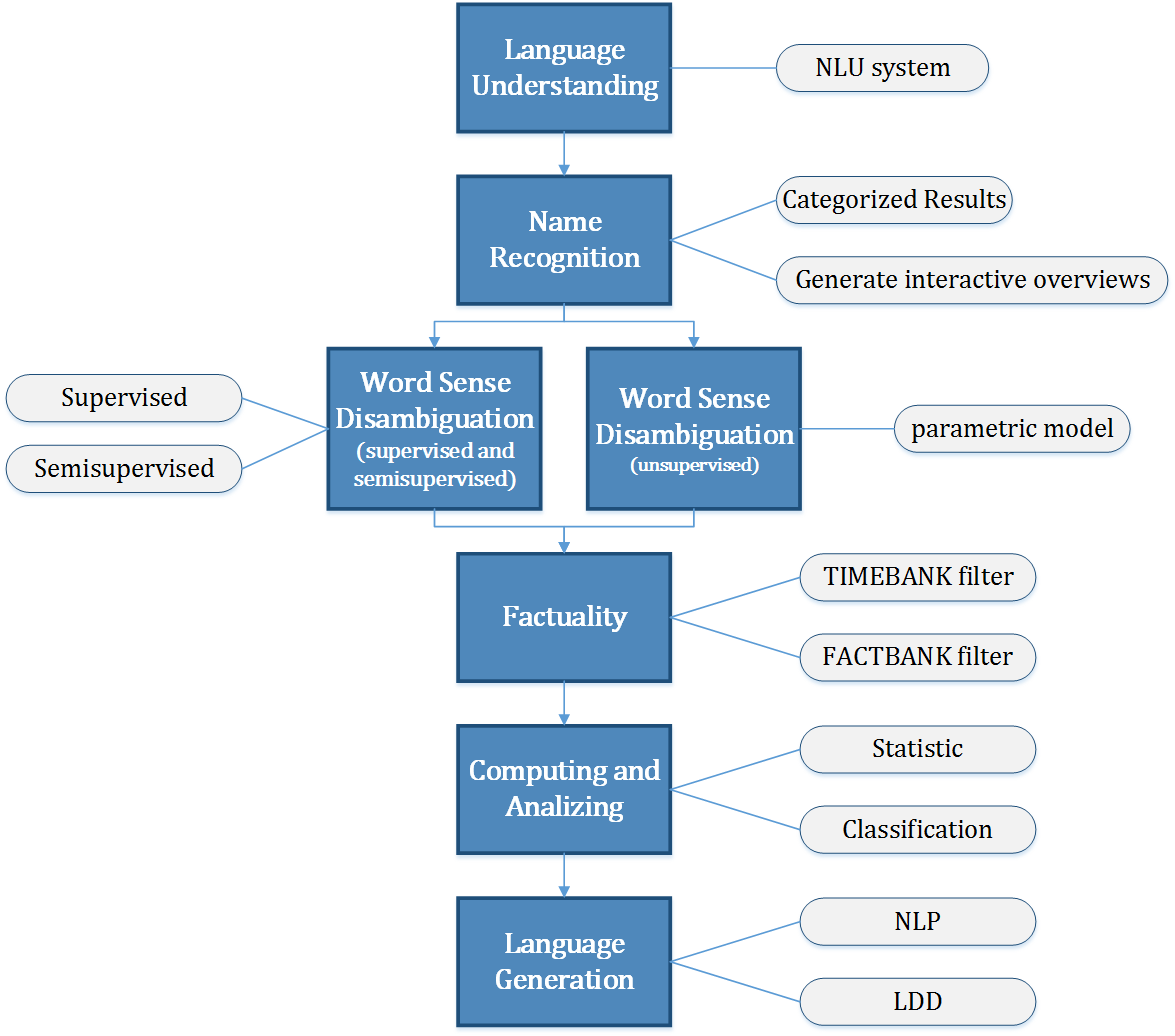
\includegraphics[width=\columnwidth]{UnionChart}
\end{center}
\end{figure}

\subsubsection*{Language understanding}
When users search for a sentence, how does the program understand certain inputs of text? 

We can build a natural language understanding (NLU) system, which uses a set of possible yes-no questions that can be applied to data items. After that, it follows a rule for selecting the best question at any node on the basis of training data by using a method for pruning trees to prevent over-training.\\ 

I believe you should read some publication and cite their work properly. Clarity in your writing should also be improved.Please take a look at it (Phat's comment)

\subsubsection*{Name Recognition}
Identifying all textual mentions of the named entities is the main goal of the name recognition mechnanism. 
The results could be a country or an animal if users search for the word, Turkey. The type is very different.

There are a lot of misunderstandings like this if users search some words which have multiply meanings. Sometimes, the results are totally unrelated and this situation is always annoying. That would be troublesome when we count frequency of a certain word to rank it.
 
Therefore, it's significantly crucial for a program to totally understand what users want by name recognition in natural language processing. The users can find out the results much quicker and can't get misunderstood.

The method to improve the above problem is "categorize the words based on different subjects,topic or genres" by using online database.Metadata is limited in digital libraries and web resources, try to enlarge them with meaningful, organized and desired categories.\cite{10.1145/1141753.1141801}

Users' exploration and overviews of information could be better supported. It will be very convenient to find the results we want and lower the possibility of misunderstanding if users are not very familiar with finding the appropriate result in specific fields.\cite{DBLP:journals/jis/NaT09} Users don't have to filter the results which are ranked by browsing frequency  popularity. Users just can obtain the information and relevance by clicking the specific categories. Also, users are able to choose multiply fields if the results include a lot of relevant fields. That's a big motivation for people to handle this problems.Plus,it could be useful and interesting if people solve the problems appropriately, even perfectly.  

A lot of online services have done similar tasks before .Thus,creating and using an online database or automated metadata creation are to be recommended. The reason why is because there are some advantages, including integrating with the other cloud service or scaling with what users need such as how to categorize the categories. It is beneficial for people who would like to create a convenient and personalized metadata.    \\

\subsubsection*{Word sense disambiguation: supervised and semi-supervised approach}

\begin{figure}[tbh]
	\begin{center}
		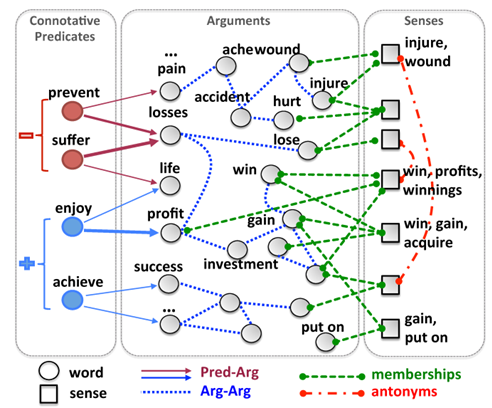
\includegraphics[width=\columnwidth]{union(WSD)}
	\end{center}
	\caption{GWord+Sense with words and senses. \label{fig1}}
\end{figure}

Word sense disambiguation (WSD) is an open problem of natural language processing and ontology. WSD identifies which sense of a word (i.e.meaning) is used in a sentence, when the word has multiple meanings(\cite{Du2013}). The solution to this problem impacts other computer-related writing, such as discourse, improving relevance of search engines, anaphora resolution, coherence, inference et cetera.

The human brain is quite proficient at word-sense disambiguation. The fact that natural language is formed in a way that requires so much of it is a reflection of that neurological reality. In other words, human language developed in a way that reflects (and also has helped to shape) the innate ability provided by the brain's neural networks. In computer science and the information technology that it enables, it has been a long-term challenge to develop the ability in computers to do natural language processing and machine learning(\cite{DBLP:journals/jis/NaT09}).

\subsection*{Supervised}

\begin{figure}[tbh]
	\begin{center}
		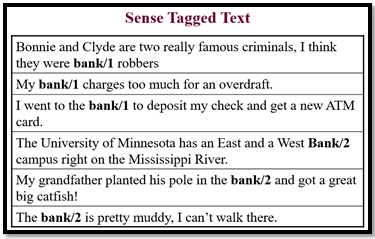
\includegraphics[width=\columnwidth]{union(sup1)}
	\end{center}
	\caption{Sense tagged text.}
\end{figure}
\begin{figure}[tbh]
	\begin{center}
		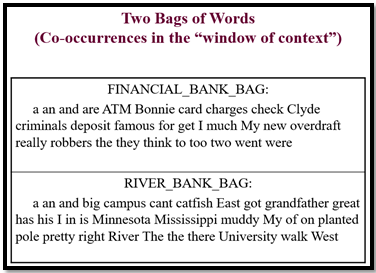
\includegraphics[width=\columnwidth]{union(sup2)}
	\end{center}
	\caption{Two bags of words.}
\end{figure}
\begin{figure}[tbh]
	\begin{center}
		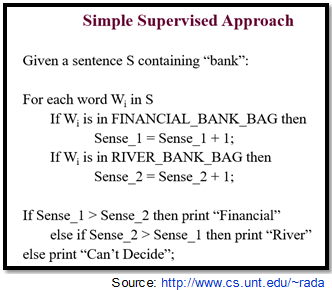
\includegraphics[width=\columnwidth]{union(sup3)}
	\end{center}
	\caption{Supervised approach.}
\end{figure}

Supervised methods are based on the assumption that the context can provide enough evidence on its own to disambiguate words (hence, common sense and reasoning are deemed unnecessary). Probably every machine learning algorithm going has been applied to WSD, including associated techniques such as feature selection, parameter optimization, and ensemble learning. Support Vector Machines and memory-based learning have been shown to be the most successful approaches, to date, probably because they can cope with the high-dimensionality of the feature space. However, these supervised methods are subject to a new knowledge acquisition bottleneck since they rely on substantial amounts of manually sense-tagged corpora for training, which are laborious and expensive to create(\citet*{Ramos-SotoBBT14}).

\subsubsection*{Semi-supervised}
Because of the lack of training data, many word sense disambiguation algorithms use semi-supervised learning, which allows both labeled and unlabeled data. The Yarowsky algorithm was an early example of such an algorithm.(\cite{Gartner201317}) It uses the 'One sense per collocation' and the 'One sense per discourse' properties of human languages for word sense disambiguation. From observation, words tend to exhibit only one sense in most given discourse and in a given collocation.

\begin{figure}[tbh]
	\begin{center}
		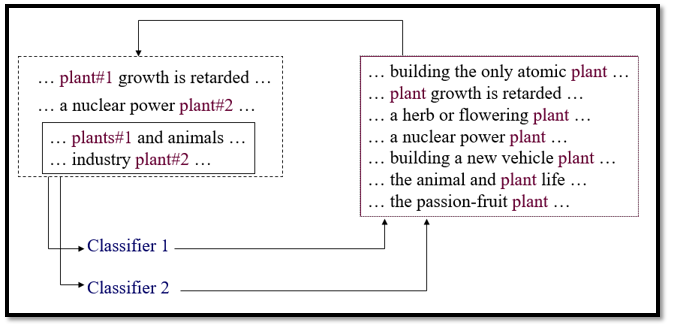
\includegraphics[width=\columnwidth]{union(semi)}
	\end{center}
	\caption{Classifier that improves over the basic classifier. \label{fig3}}
\end{figure}

The bootstrapping approach starts from a small amount of seed data for each word: either manually tagged training examples or a small number of surefire decision rules (e.g., 'play' in the context of 'bass' almost always indicates the musical instrument). The seeds are used to train an initial classifier, using any supervised method. This classifier is then used on the untagged portion of the corpus to extract a larger training set, in which only the most confident classifications are included. The process repeats, each new classifier being trained on a successively larger training corpus, until the whole corpus is consumed, or until a given maximum number of iterations is reached(\cite{Blascheck2016}).

Other semi-supervised techniques use large quantities of untagged corpora to provide co-occurrence information that supplements the tagged corpora. These techniques have the potential to help in the adaptation of supervised models to different domains.\\
Also, an ambiguous word in one language is often translated into different words in a second language depending on the sense of the word. Word-aligned bilingual corpora have been used to infer cross-lingual sense distinctions, a kind of semi-supervised system (\cite{Cheslow2014}).

\subsubsection*{Unsupervised}
Word Sense Disambiguation (WSD) is related to Natural Language Processing and is linked with computational languages.People introduced it when they felt the need of complex problems like: machine translation, information retrieval, speech processing and text processing etc. The use of WSD is focused on determining the sense of word which is used in a problem by using that word in a particular context. Inspite of having a greater number of existing disambiguation algorithms ,WSD still has an open problem with the three main parts of the WSD methods being considered by literature: supervised, unsupervised and knowledge based disambiguation \cite{Guenther200312}.

Unsupervised WSD which rely on single writing can be approached by the use of Naive Bayes' model, which mainly focuses on it. In this model, a number of sentences are used which contains a particular word which has several meanings. The main goal is to divide those words into a specified number of sense groups.
The Naive Bayes model applied mathematically entirely focuses on the issue of feature selection, which describes its two types:

\begin{enumerate}
	\item Pedersen and Bruce local type features.
	\item WordNet-based feature selection.
\end{enumerate}

Apart from the above mentioned model, the web can act as a corpus too, where it searches words which are relevant and distinctive for the target word, which makes it more appropriate in searching particular words' meaning.The Supervised approaches make use of information from labeled training data while the Unsupervised ones rely on the UMLS metathesarus.

So, this background focuses mainly on the issues of feature selection for unsupervised WSD performed with an underlying Naive Bayes model.



\subsubsection*{Factuality}
In the process of producing metadatas, which are should be the most precise information and representing the text, validity of such metadata must be checked. Therefore tools for fact checks are developed based on linguistic techniques.  The tool could detect facts and excludes authors' subjective opinions \cite{agerri2015big}. From this paper's perspective, the two main set of tools having such functions is TIMEBANK and FACTBANK.

TIMEBANK was first proposed in \cite{pustejovsky2003timebank}. The idea was based on that English language has different tenses which could be exploited as signals for fact check. An example as below could help to clarify the ideas. Let's examine these sentence:

\begin{itemize}
	\item I will go to Chimei museum tomorrow.
	\item Chimei museum is near Tainan District.
	\item I was in UK in 2012.
\end{itemize}

The first sentence is simple future tense which implys something has never actually happened, the second sentence is simple present tense which can directly imply facts, and the last sentence is in simple past tense which is about something already happened (which is facts), but is no longer a fact right now -- so such fact must be used with caution. 

In addition to TIMEBANK, many other tools can be another filter for fact extraction. The reason for introducing such tool is that even scientific research articles can be glittering with subjective comments, opinions or even assumption from authors \cite{schultze2000confessional}. \cite{dave2003mining} identify words, clauses and phrases that show emotional state of the authors. The choice in expression of facts could also be a helpful indicator to show whether authors are subjectively supporting a cause, an opinion and so on \cite{wiebe2005annotating}. Among these mentioned approaches, this paper highly favors creation a kind of thesaurus compiled of linguistic signaling for non-factually statements such as FACTBANK, which is built by \cite{sauri2009factbank}. Following example shows how subjective statements can be picked out.

\begin{itemize}
	\item Channelization would guarantee high flow velocity in rivers, more flooding and consequent degradation of riparian community (1a)
	\item Funding agencies would be happy with big entrepreneurs, instead of small and medium enterprises. (1b)
	\item Tolerance to dictatorship would has negative influences on anarchist movement (2a)
	\item Tolerance to dictatorship would doom anarchist movement. (2c)
\end{itemize}

It is easy to find in statement (1a) is an absolute fact. Statement (1b) is however affected by emotional state of authors. After re-writing (1b) into: Funding agencies lend more money with lower interest rate to big entrepreneurs, instead of small and medium enterprises, sentence (1b) become a face-based statement. In another case, statement (2a) is a fact-based statement while in statement (2b), authors are stressing their dislike toward dictatorship.

Fact checks in language generation is a new field but many useful tools have been developed. Each of them has their own function and could complement each others. In the limit of this study, we are using both of TIMEBANK and FACTBANK together for fact check.

\subsubsection*{Computing and analyzing}
This is actually not a background. It's more suitable to methodology section.

\ul{I suggest we should use the Python language to complete this task. It can easily compute and analyze words in the articles. Python can compute and analyze by separating connected words. Therefore, readers can know what do the words mean when they are reading the articles .}

\subsubsection*{Direction}
\ul{In order to highlight the focus of the article ,the special and important words in the article need to be found mostly. The article will promote these words to make the article's main point prominent. Compute all the words in the article and show the number of occurrences of most rankings. By these words ,the analyzer know which words in the article should be analyzed.}


Same as above, you continued to discuss your methodology without showing the background. 
\subsubsection*{Operate}
\begin{itemize}
	\item distinguish: distinguish all the words
	\begin{center}
		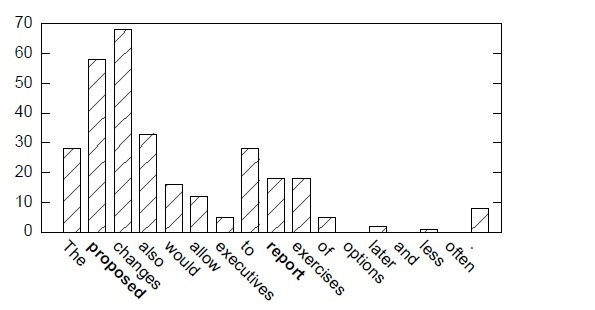
\includegraphics[width=0.8\columnwidth]{union_01.jpg}
	\end{center}
	\item classification: Divided into four categories\\ 	
	(a)  Word Count $>$ 15\\
	(b)  15 $>$ Word Count $>$ 10\\
	(c)  10 $>$ Word Count $>$5\\
	(d)  5 $>$Word Count	
	\begin{center}
		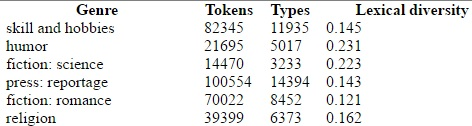
\includegraphics[width=0.8\columnwidth]{union_02.jpg}
	\end{center}
	\item search : Search Word repetition rate
	\item statistics: Count the repetition rate of words
	\item sort: Show the number of rankings
\end{itemize}
Show the number of rankings \\

\subsubsection*{Language generation}
In the part of language generation, we would introduce two methods which are used generally in this field: then, what are they? It's better to list them there as it help you write more clearly.
Natural language generation: Natural language generation is one branch of natural language processing. The goal is generating the words human being using via machine automatically. To imply this technique, six basic activities which conclude content determination, discourse planning, sentence aggregation, lexicalization, referring expression generation and linguistic realization are constructed. \cite{aramossoto2016onthe}. Some of the activities are mentioned above. The advantage of this technique is that it is flexible, since there is no standardization. But it also has the difficulty in the implication of this technique.\cite{aramossoto2016onthe}

Linguistic description of data: Linguistic description of data (LDD) is a concept that applied the fuzzy set theory in the linguistic field. At the beginning, comparing to the NLG field, it is a newer technique to solve the problem of language generation. However, the basic steps of LDD have been built. The four main parts in this technique are input data, linguistic variable, fuzzy quantifiers and evaluation criteria \cite{aramossoto2016onthe}. Some of them are similar to the concept. The advantage of this technique is that it has been implied in many fields like weather forecast \cite{Ramos-SotoBBT14}. Also, many practical methods have been proposed. However, it still has a long way to go.

These two techniques are usually combined together nowadays. The concept of NLG and the practical approach of LDD could be used in the same time to provide the better performance in language generate field.

\newpage % Ends the current page and causes all figures and tables to be printed

	\section{Methods}
	\label{Methods}
	
	\section{Results and discussion}
	\label{Results and discussion}

	\section{Conclusions and future work}
	\label{Conclusions and future work}

	%%%%%%%%%%%%%%%%%%%%%%%%%%%%%%%%%%%%%%%%%%%%%%%%%%%%%%%%%%%%%%%%%%%
	% References
	%
	% I'm using Mendeley Desktop with library.bib
	%%%%%%%%%%%%%%%%%%%%%%%%%%%%%%%%%%%%%%%%%%%%%%%%%%%%%%%%%%%%%%%%%%%		
	\bibliographystyle{agsm}
	\bibliography{library}	
	\clearpage 
\end{document}  
